\section{Methodology for the SLR}
For this SLR, we followed the guidelines provided by Kitchenham \cite{kitchenham2004procedures}. Figure \ref{fig:slr-overview} presents the protocol that we have designed to conduct the SLR.
\begin{enumerate}
    \item Firstly, we formulate the research questions that guides this SLR, and further identify which information to be extracted from the literature.
    \item Nextn, we defined the search keywords aimed at retrieving the broadest possible set of relevant publications within the scope of the SLR.
    \item To limit our studies on highly relevant papers, we apply exclusion criteria to filter out publications of likely interest.
    \item Finally we perform a lightweight backward-snowballing on the selected publications. The resulting set of studies are referred to as the primary publications.
\end{enumerate}


\subsection{Research Questions}

\textbf{RQ1: What are the purpose of these static analysis techniques/optimizations?}
With this research question, we will survey the various optimization techniques in static analysis. \\
\textbf{RQ2: How are the analyses designed and implemented?} \\
In this research question, we conduct a detailed study of the analysis that have been developed. It also includes several sub-questions:\\
\textit{RQ2.1} What fundamental techniques are used for by this static analysis optimization?\\
\textit{RQ2.2} What sensitivity features are applied?\\
\textbf{RQ2: Are the research outputs publcly available?}
We aim to investigate whether the developed tools are open-source or publicly available, reproducible, and easily accessible for use by other practitioners. \\
\textbf{RQ3: What challenges remain to be addressed?}
This question addresses issues that have not yet received significant research attention. It also examines how the focus of the research has evolved over time. 
Additionally, it helps in identifying the research gaps in the current knowledge base, and aims to understand the emerging trends and shifts in priorities within the field.

\subsection{Search Strategy}
This section discusses the keywords we used in our search and the datasets employed to find the relevant publications.

\subsubsection{Search Keywords}
We used the PICOC strategy to develop our search term. Since the \textbf{Intervention (I)} and \textbf{Comparison (C)} terms were not relevant to our scope, they were left empty.

Each of the terms from \textbf{ Population (P)}, \textbf{Outcome (O)}, and \textbf{Context (C)} formed a seperate line in the search string. The final search string was constructed by logically combining these lines, using \textbf{AND} to connect different categories (P, O, C), and \textbf{OR} within each category for synonyms or related terms.
i.e., s =: P \textbf{AND} O \textbf{AND} C \\
Table \ref{tab:picoc_terms} shows the actual keywords we used, which were derived from a manual investigation of relevant publications.

\begin{table}[h]
    \centering
    \begin{tabular}{cc}
    \toprule
    \textbf{PICOC} & \textbf{Search Terms} \\
    \midrule
    P & \text{"control-flow analysis", "data-flow analysis", "static analysis"} \\
    \midrule
    O & \text{"accuracy", "efficiency", "memory usage", "overhead", "performance", "precision", "scalability", "speedup"} \\
    \midrule
    C & \text{"control-flow analysis", "data-flow analysis", "static analysis"} \\
    \bottomrule
    \end{tabular}
    \caption{Search Terms}
    \label{tab:picoc_terms}
\end{table}

\begin{figure}
    \centering
    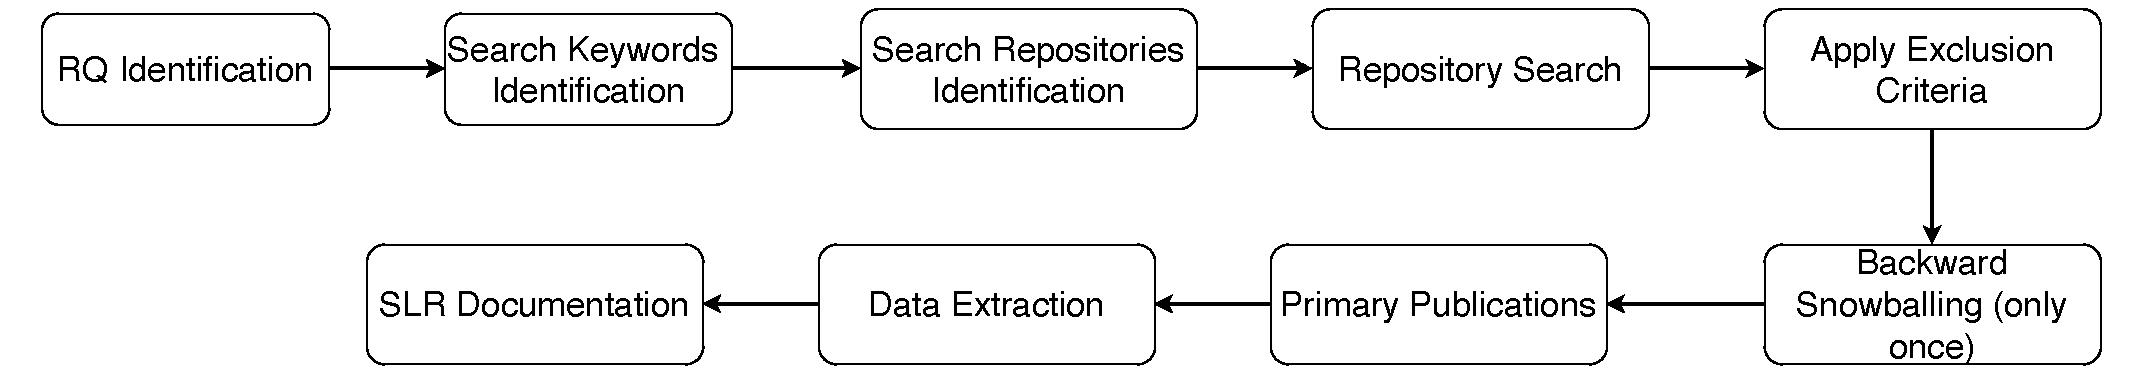
\includegraphics[width=1\linewidth]{figures/SLR.drawio.pdf}
    \caption{An overview of the systematic literature review process.}
    \label{fig:slr-overview}
\end{figure}

\subsubsection{Search Datasets}
We used four well-known repositories, namely ACM Digital Library \footnote[1]{http://dl.acm.org/}, IEEE Xplore Digital Library \footnote[2]{http://ieeexplore.ieee.org/}, Springer Link \footnote[3]{http://link.springer.com/}, and Google Scholar \footnote[4]{https://scholar.google.com/}. Some of these repositories impose restrictions on the amount of search result metadata that can be downloaded. For instance, Google Scholar does not allow frequent search requests from a single device via its API. To overcome this limitation, we used Publish or Perish \footnote[5]{https://harzing.com/resources/publish-or-perish}, a tool that helps retrieve academic documents from Google Scholar. Similarly, Springer Link limits metadata downloads to the first 1,000 search results. However, our search query yielded approximately 10,000 results on this repository. Manually downloading metadata in batches would have been tedious and time-consuming. To handle this efficiently, we used Python scripts to extract data from Springer Link, IEEE Xplore, and ACM Digital Library.

\subsubsection{Exclusion Criteria}
The search terms we used were quite broad, resulting in an exhaustive list of publications. Due to this broad scope, many papers in the search results may be irrelevant to our review. To refine our selection and exclude non-relevant papers, we applied specific exclusion criteria, which are detailed below:

\begin{enumerate}
    \item Given that the majority of scientific publications today are in English, we exclude all non-English papers from our review.
    \item Papers under 5 pages in double-column format or under 7 pages in LNCS single-column format were excluded. Additionally, papers exceeding 30 pages in LNCS single-column format were also excluded.
    \item If multiple papers described the same or similar approaches, we included only the one with the most comprehensive description. For example, an extended journal paper \cite{lu2021eagle} was selected over its shorter conference version \cite{lu2020precision}.
    \item Papers lacking sufficient technical details about their approaches were excluded.
    \item Papers that did not focus on optimizing static analysis itself were excluded. For example, papers that use static analysis to optimize the analyzed program were considered out of scope and excluded.
    \item Papers that focus on dynamic or hybrid analysis were excluded.
\end{enumerate}


\subsubsection{Primary publications selection}
Table \ref{tab:summary_slr} summarizes the results of the search process. For each paper, we first reviewed the title and keywords to determine its relevance to our use case. If the relevance was unclear, we proceeded to read the abstract. If the abstract was still insufficient to make a decision, we skimmed the paper to assess its suitability.
\todo{Usually here we should discuss how many reviewers did read the paper, and how did you overcome the inconsistencies the results?}
In the end, we got \primarypapers papers in total.

\subsubsection{Backward snowballing}
To ensure the completeness of our study and to capture relevant works not identified through our initial search terms, we conducted a lightweight backward snowballing process, performed only once.
The objective was to identify additional papers cited by our initially selected primary publications that align with the scope of our study.
Manual snowballing process it tedious and time consuming, so we developed a series of python scripts to automate and streamline the process.
First, We used pdfx \footnote{https://github.com/metachris/pdfx} to extract the text from the pdf and then retrieved the references from the extracted text.
Subsequently, additional scripts were used to filter out papers which fell outside the defined year boundary of our study scope.
Furthermore, we used python scripts to extract keywords from the paper, and eliminated those that did not align with the scope of our review.
After the automatic filtering stage, we manually reviewed the titles and abstracts of the remaining references. 
Papers found relevant to the scope of study, and not already included in our primary publications set were added to the final list of primary publications.
The relatively high number of additional papers identified through backward snowballing can be attributed to the fine-grained terms used by the original studies, which were not fully covered by our broader search strategy.
For instance, many papers contains keywords such as context-sensitivity, context, parallel processing, call graph, call site sensitivity, which, although highly relevant, were not explicitly included in our original search queries.
Our initial search term aimed for broader coverage, while snowballing allowed us to capture these more granular studies.


\begin{table}
    \begin{tabular}{lccccc}
    \toprule
    Source                         & IEEE & ACM  & Springer & Google Scholar & Total \\
    \midrule
    Search Results                 & 5561 & 3195 & 3980     & 1000           & 13736 \\
    Script verification (keywords) & 225  & 450  & 45       & 97             & 817   \\
    After Reviewing Title          & 125   & 136  & 13       & 43             & 317   \\
    After Reading Abstracts        & 117  & 30   & 22       & 2              & 171   \\
    After Skimming                 & 72   & 22   & 3        & 20             & 117   \\
    After Final Discussion         &      &      &          &                & 96    \\
    Backward snowballing           &      &      &          &                & 28    \\
    Total                          &      &      &          &                & 124   \\ 
    \bottomrule
    \end{tabular}
    \caption{Summary of the Primary Publications Selection Process}
    \label{tab:summary_slr}
\end{table}

\subsubsection{Primary publication Selection}
In this section, we present the final selection results of the primary publications, as summarized in Table \ref{tab:summary_slr}.
The first row (search results) shows statistics on the papers retrieved using the keywords defined in the previous section. Through this repositories search, we collect metadata such as paper title, abstracts and additional relevant information.
We introduced a second filtering step, due to the inconsistent and often flawed results of the "advanced" search feature of the search repositories, where the search results are oftern inaccurate resulting in the set of irrelevant and noisy results. 
After performing the second step (represented in row 2), the number of potential relevant papers are significantly reduced.

    